\section{Déploiement}

Pendant le développement des différents Générateurs de Code, nous avons pu utiliser les outils proposés par \kweclipse afin de configurer statiquement le répertoire cible des fichiers à générer lors de l'exécution desdits générateurs. Cette méthodologie nous a permis de définir un Projet \kwplay dédié comme cible de la génération, afin d'effectuer des tests rapidement, sans qu'il ne soit requis de reconfigurer la génération après chaque modification. Le système en place nous a donc permis de tester chaque générateur (pour Entity, SOA, et Cinematic) indépendament.
\\\\
Il n'était cependant pas concevable d'utiliser la même méthodologie pour une \guim{mise en production} du générateur \kwplay. En effet, il n'est pas concevable d'obliger un utilisateur à configurer et lancer manuellement chaque \guim{sous-générateur}, car ceux-ci sont complémentaires (à l'exception peut-être de la génération des WebServices). De plus, il faut dispenser l'utilisateur d'une configuration fastidieuse, et trouver un système plus ergonomique pour que ce dernier puisse lancer rapidement une génération de code.

\subsection{Regroupement des différents générateurs de code}

La première étape du déploiement a été de réunir les différents \guim{sous-générateurs} en un seul générateur principal. Pour cela, nous avons choisi de créer un Méta-Modèle abstrait défini pour pouvoir contenir tout type de Modèle. Ainsi, nous avons pu encapsuler chaque Modèle utilisé - en l'occurence, Entity, SOA et Cinematic - en un seul Modèle \guim{Application}.
\\
Nous avons ensuite modifié la manière dont les générations sont lancées afin que le Modèle unique soit automatiquement parcouru afin d'y retrouver chaque Modèle pour ainsi lancer les générateurs correspondant.

\begin{figure}[htb]
  \centering
  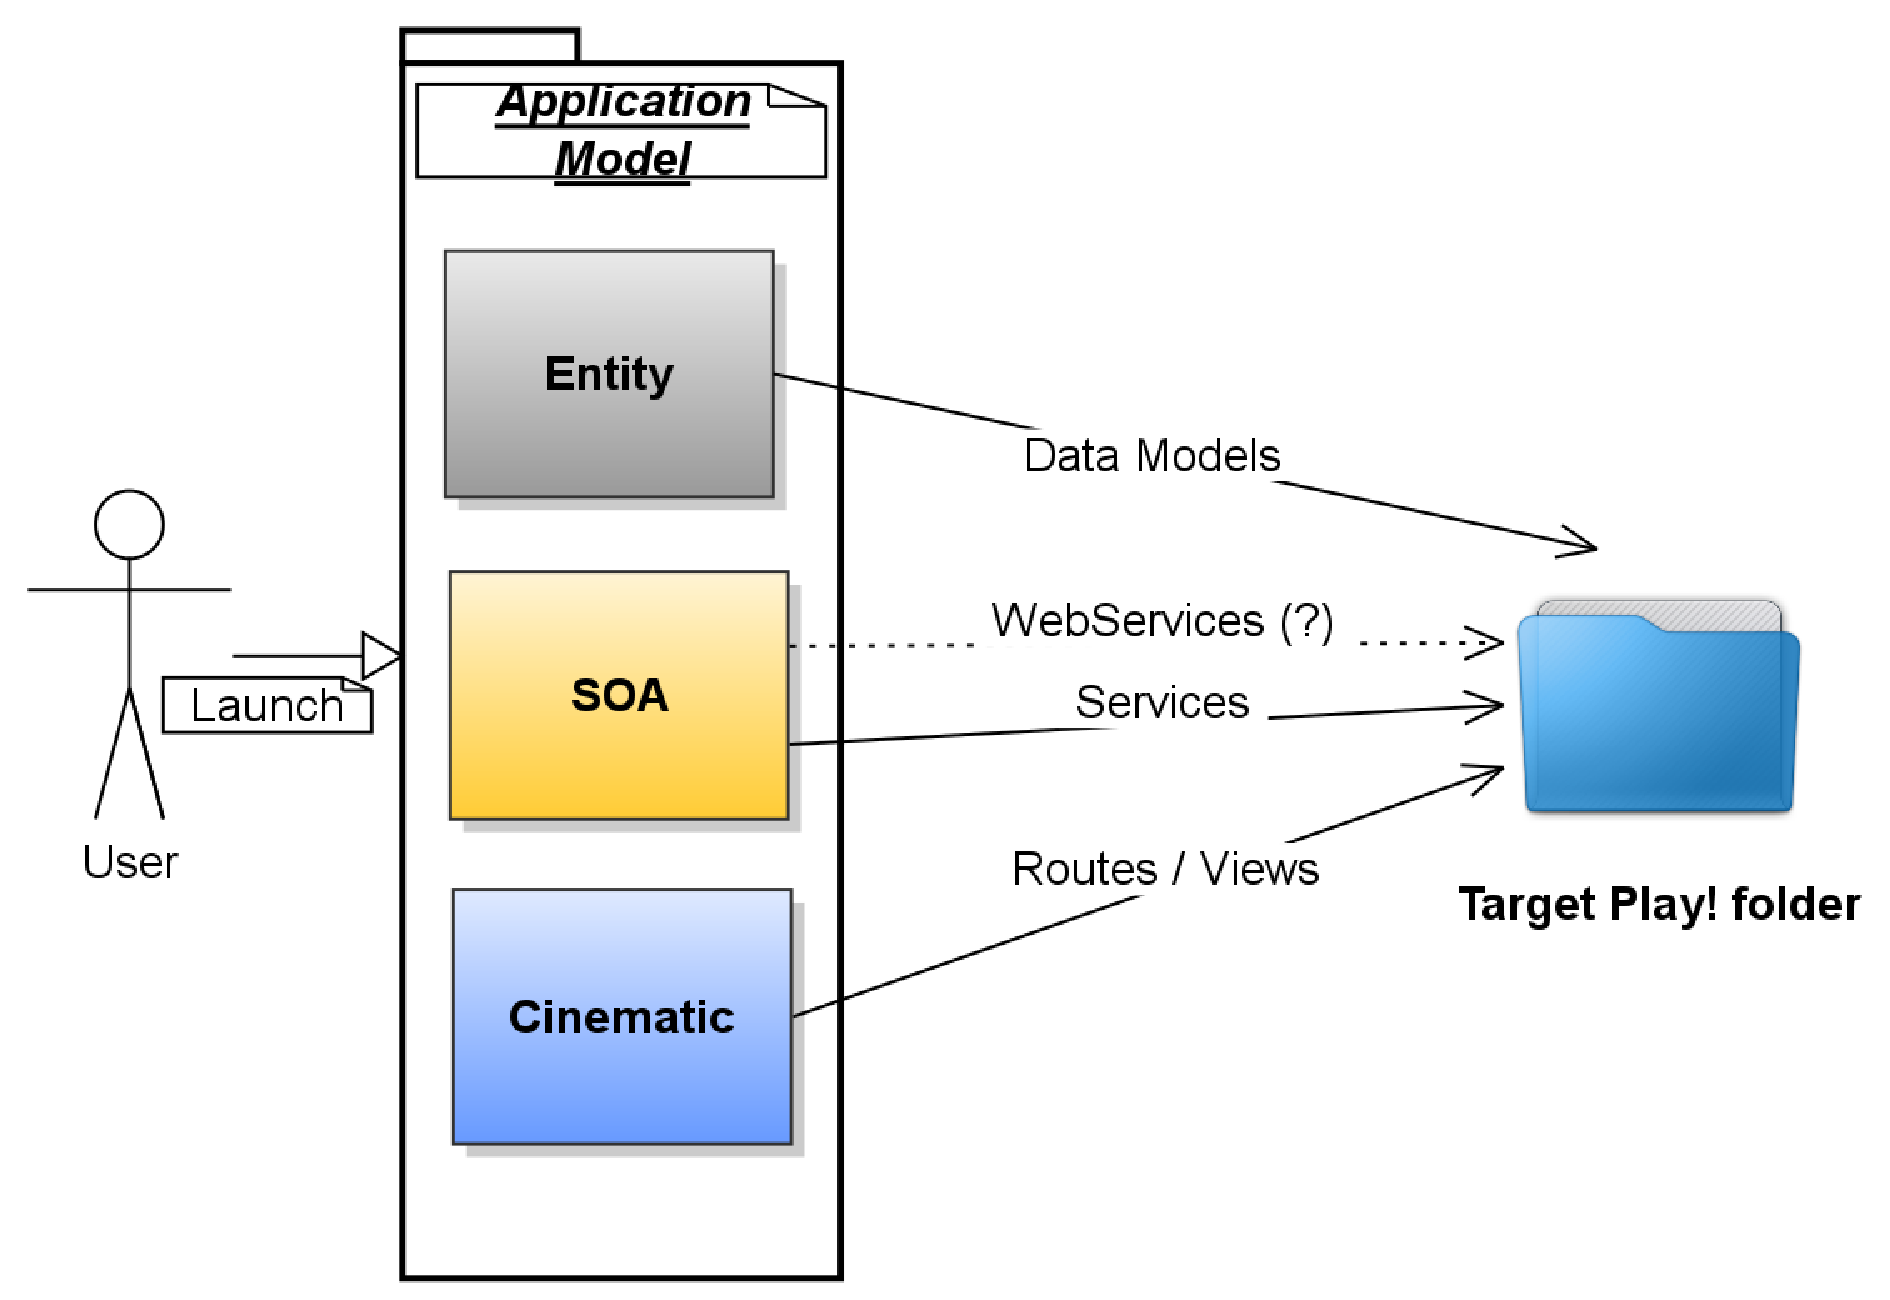
\includegraphics[scale=0.4]{img/application_scheme.eps}
  \caption{Structure de notre Modèle \guim{Application}}
  \label{fig:acceleo}
\end{figure}
\subsection{Interface Utilisateur}

\kwacceleo embarque une grande quantité d'outils pour faciliter le déploiement des générateurs de code. Nous avons donc pu générer automatiquement une interface utilisateur. Cette interface se présente sous forme d'un Plugin \kweclipse qui permet d'ajouter automatiquement un menu conextuel \guim{Générer application Play!} lorsqu'un clic-droit est effectué sur un fichier Modèle.
\\
Afin de rendre la génération plus adaptée aux besoins des utilisateurs, nous avons légèrement modifié le code de ce Plugin afin que l'utilisateur puisse sélectionner rapidement le dossier de destination du code à générer. Cela nous a également permis d'ajouter une \textit{Checkbox} (case à cocher) demandant à l'utilisateur s'il souhaite - ou non - générer le code relatif aux WebServices du site \kwplay.

\begin{figure}[htb]
  \centering
  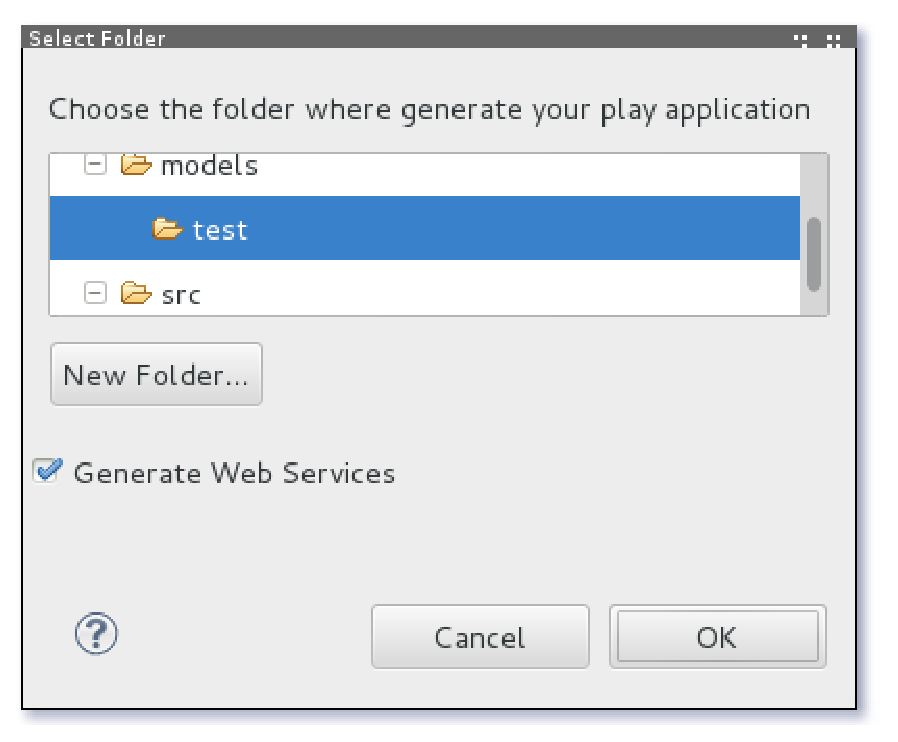
\includegraphics[scale=0.55]{img/screen_ui.eps}
  \caption{Interface Utilisateur pour le lancement du générateur}
  \label{fig:acceleo}
\end{figure}